\documentclass[utf8]{beamer}

%\usepackage[german]{babel}
\usepackage{ngerman}
\usepackage{xcolor}
\usepackage{graphicx}
\usepackage{tikz}
\usepackage{caption}
\usepackage{subcaption}

%Für den Header notwendig!
%\usepackage[percent]{overpic}

\usepackage{hyperref} % für korrekte Links

% Theme
\input{design_latex-template/beamerthemeFOSSAG.sty}


\title{Informatik AG}

\author{FOSS-AG}
%\titlegraphic{\includegraphics[width=\textwidth,height=\textheight]{/home/innay/repos/vorlage_corporate-design/png/basis/ohne-text/500px.png}}
\institute[FOSS AG]{
\includegraphics[height=0.19\textheight]{img/logo_text-voll-transp.png}\hspace{0.5cm}
	
\includegraphics[width=0.45\textwidth]{img/AIDO_Logo_farbig_cmyk_breit.png}
	%\textbf{F}ree and \textbf{O}pen \textbf{S}ource \textbf{S}oftware \textbf{AG}
}
%


\date{6. Februar 2018}

\begin{document}
	\begin{frame}
		\titlepage
	\end{frame}

	\begin{frame}{FOSS-AG - Wer, was und warum?}
			\centering{
\includegraphics[height=0.3\textheight]{img/logo_text-voll-transp.png}}
		\begin{itemize}
			\item (Informatik-)Studierende
			\item Beschäftigung mit quelloffener Software und Linux
			\item Veranstaltungen
			\item Interesse wecken
			\item Informieren über die Relevanz von quelloffenen Programmen im Alltag
		\end{itemize}
	\end{frame}
	\begin{frame}{Was wir die nächsten Wochen machen}
		\begin{figure}
			\begin{subfigure}{0.45\textwidth}
				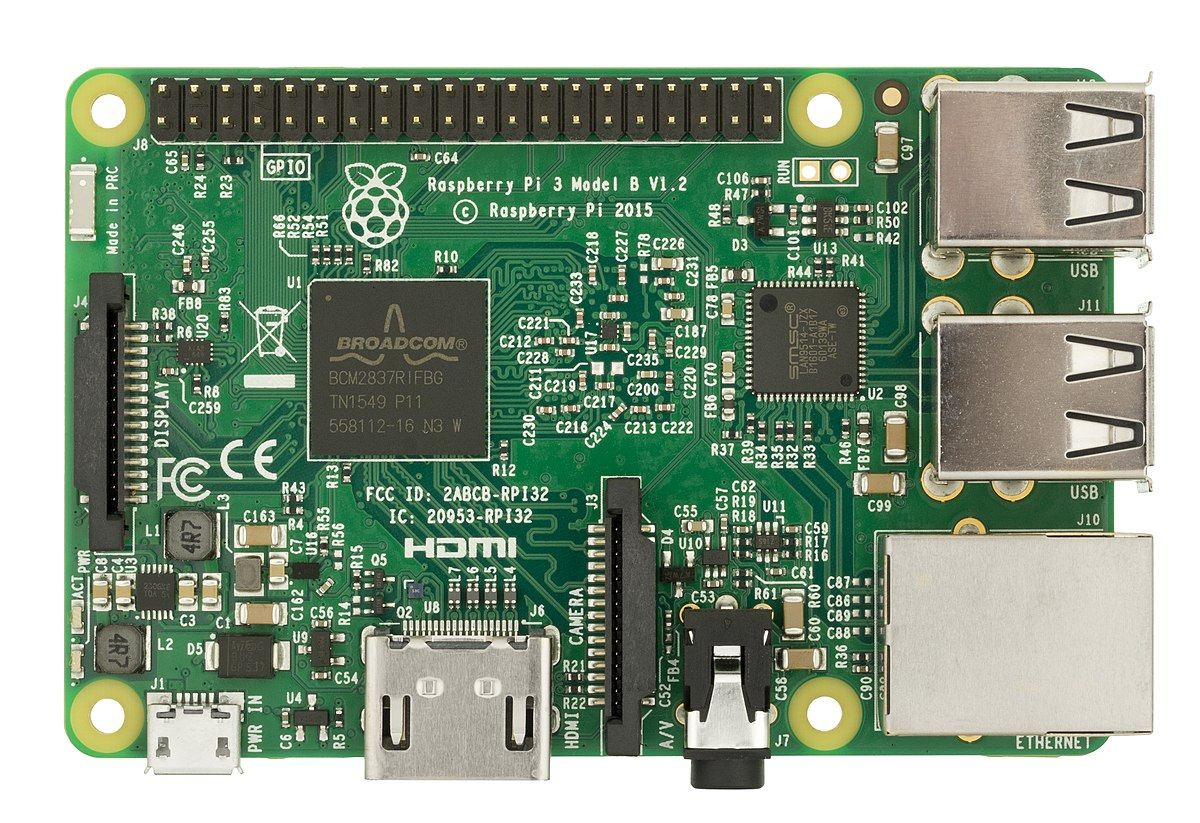
\includegraphics[width=\textwidth]{img/1200px-Raspberry-Pi-3-Flat-Top.jpg}
			\end{subfigure}
			\begin{subfigure}{0.45\textwidth}
				
\includegraphics[width=\textwidth]{img/Python_logo_and_wordmark200dpi.png}
			\end{subfigure}
		\end{figure}
		\begin{itemize}
			\item Raspberry Pi kennenlernen
			\item Erste Schritte in Python
			\item Minecraft modifizieren
		\end{itemize}
	\end{frame}
	
	\begin{frame}{Linux - freie Software, freies Betriebssystem}
	\centering
\includegraphics[width=0.3\textwidth]{img/Tux-simple.png}\\
		\begin{itemize}
			\item Freies Betriebssystem
			\item Gut zum Entwickeln
			\item Läuft auf den unterschiedlichsten Geräten
		\end{itemize}
	\end{frame}
	
	\begin{frame}{Vorteile des Raspberry Pi}
		\centering
\includegraphics[width=0.25\textwidth]{img/Raspberry_Pi_Logo.png}
		\begin{itemize}
			\item Günstig
			\item Relativ leistungsfähig
			\item Linux
			\item Quasi vollwertiger PC nur in klein
		\end{itemize}
	\end{frame}
	
	\begin{frame}{Raspberry Pi}
		\centering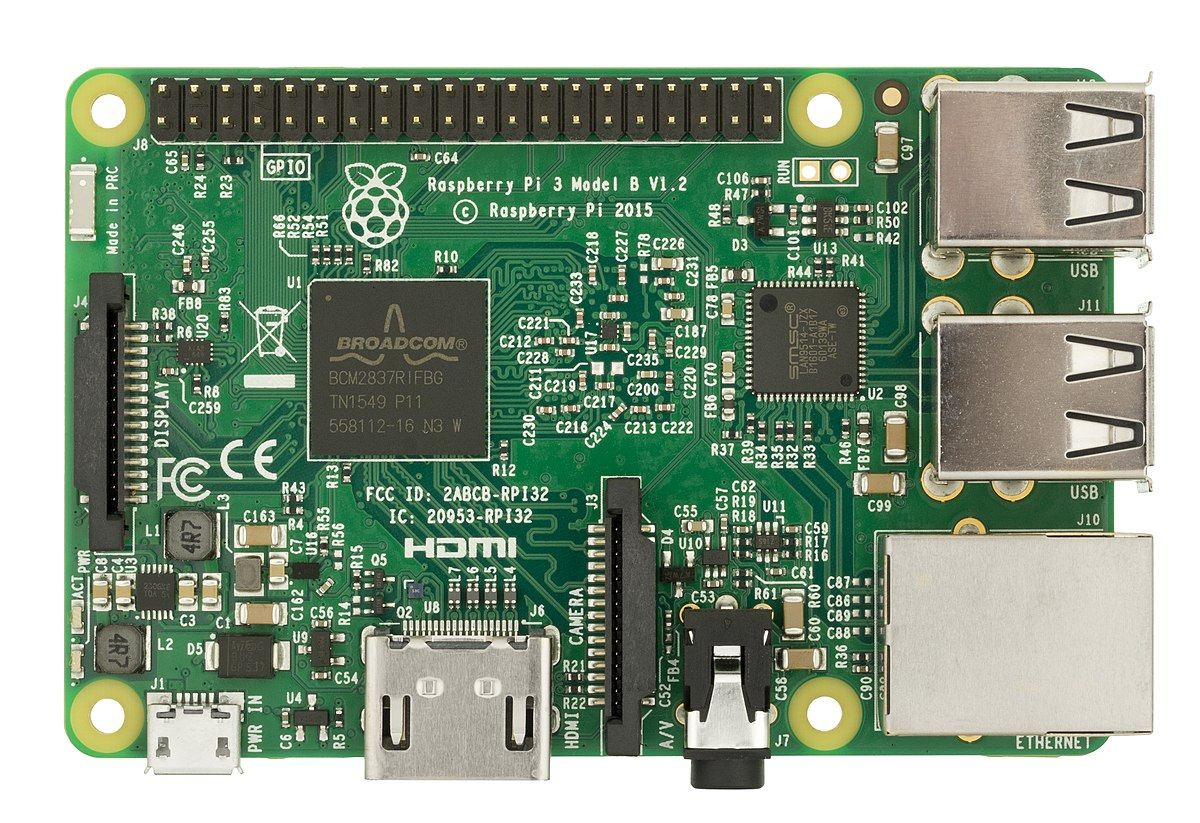
\includegraphics[width=\textwidth]{img/1200px-Raspberry-Pi-3-Flat-Top.jpg}
		
		%\tableofcontents[hideallsubsections]
	\end{frame}
	
	%\section{Die FOSS-AG}
	
	
	%\input{Einleitung.tex}
	
	%\section{Thema}
	%\input{blah.tex}
	
	
\end{document}